\chapter{Θεωρητικό Υπόβαθρο}
\label{chapter:theory}

Στο κεφάλαιο αυτό παρουσιάζονται ορισμένα βασικά θεωρητικά στοιχεία για την πλήρη κατανόηση της διπλωματικής αυτής εργασίας. Πρώτα, γίνεται αναφορά στα OGM και πώς αυτά αποθηκεύουν την πληροφορία του χώρου. Μετά αναλύεται το Γενικευμένο Διάγραμμα Voronoi. Τέλος, παρουσιάζονται οι αλγόριθμοι Brushfire, Dijkstra και Hill Climbing. 
% και τα Support Vector Machines.


\section{Occupancy Grid Map (OGM)}
\label{section:ogm}

Η αναπαράσταση του χώρου μετά από την εφαρμογή του αλγορίθμου SLAM\footnote{\href{http://wiki.ros.org/gmapping}{http://wiki.ros.org/gmapping}} πραγματοποιείται με την χρήση \emph{χαρτών πλέγματος κατάληψης} (Occupancy Grid Maps) στους διδιάστατους χώρους, όπως περιγράφεται από τους Wolf και Sukhatme \cite{ogm2005}. Αναπαρτιστά τον χώρο ως ένα σύνολο τετραγωνικών κελιών, στα οποία αποθηκεύεται πιθανότητα η κατάληψης τους. Το κάθε κελί μπορεί να πάρει τρεις διαφορετικές καταστάσεις που αντιστοιχούν στις παρακάτω τιμές:
\begin{itemize}
    \setlength\itemsep{-0.2em}
    \item 100 όταν είναι κατειλημμένο (obstacle).
    \item 0 όταν είναι ελεύθερο (free space).
    \item -1 όταν είναι άγνωστο το περιεχόμενο του σημείου (unknown).
\end{itemize}
Κατά τη διαδικασία του SLAM διαβάζονται οι μετρήσεις του αισθητήρα που χρησιμοποιείται και όσο αυτός δείχνει ότι μια θέση είναι ελεύθερη τόσο η τιμή του κελιού της στο OGM θα μειώνεται έως και την τιμή 0, ενώ αντίστοιχα όσο θα δείχνει ότι μια θέση είναι κατειλημμένη, τόσο η τιμή στο κελί του OGM θα αυξάνεται μέχρι την τιμή 100. Με αυτόν τον τρόπο ορίζεται η πιθανότητα κατάληψης των κελιών.

Στο \autoref{fig:sparse_3_ogm} παρουσιάζεται ένα OGM ενός χώρου που προέκυψε μετά από προσομοίωση SLAM στο Gazebo. Τα εμπόδια έχουν μαύρο χρώμα, ο ελεύθερος χώρος άσπρο και ο άγνωστος γκρι.
\begin{figure}
    \centering
    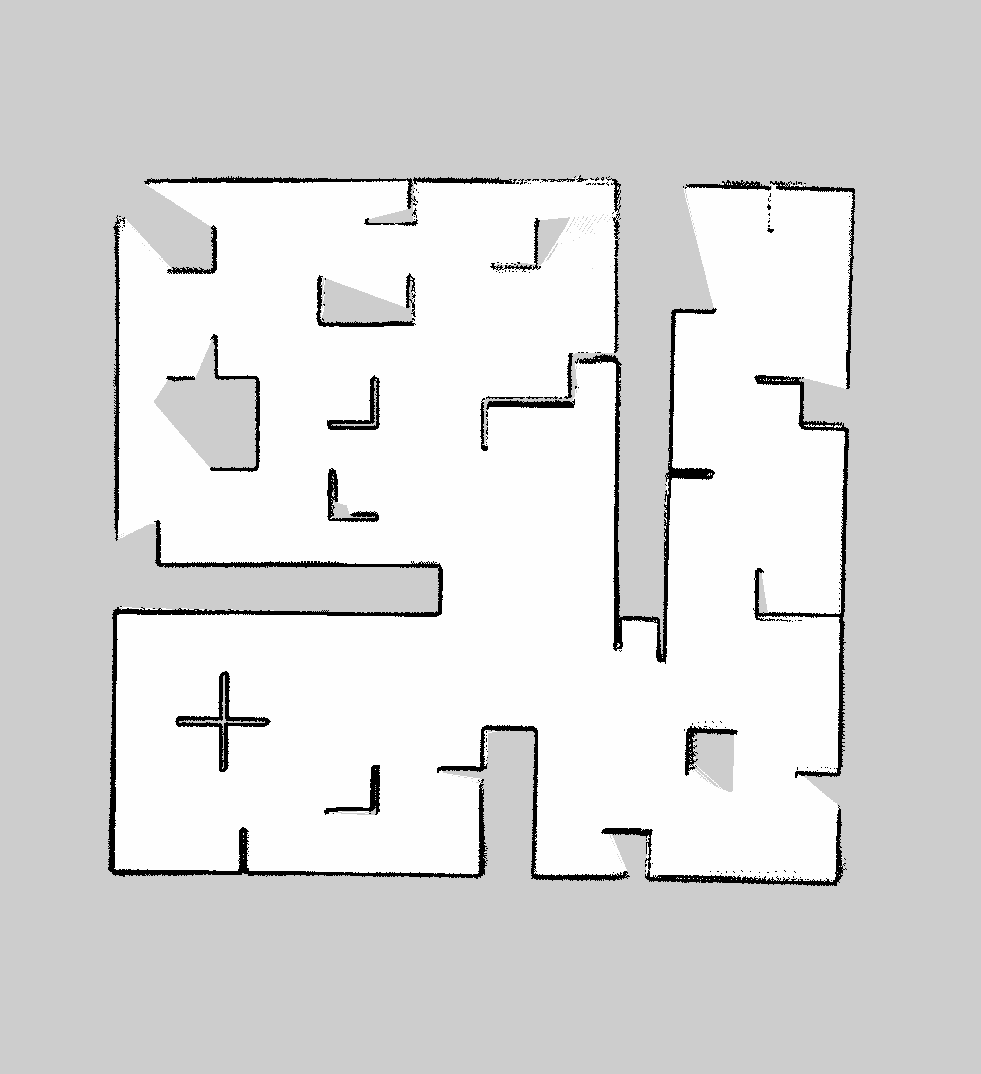
\includegraphics[width=0.5\textwidth]{./images/chapter3/sparse_3.png}
    \caption{Παράδειγμα ΟGM εικονικού χώρου}
    \label{fig:sparse_3_ogm}
\end{figure}

\section{Generilized Voronoi Diagram (GVD)}
\label{section:gvd}


Το \emph{Γενικευμένο Διάγραμμα Voronoi} αποτελεί μια μέθοδο διαχωρισμού ενός χώρου σε επιμέρους περιοχές. Ο διαχωρισμός αυτός πραγματοποιείται με βάση τις αποστάσεις κάθε σημείου του χώρου από ένα υποσύνολο σημείων, σαφώς καθορισμένων από την αρχή της διαδικασίας. Οι τελικές περιοχές ονομάζονται κελιά Voronoi.
Στο \autoref{fig:euclidean_voronoi} παρουσιάζεται ένα παράδειγμα ευκλείδιου διαχωρισμόυ του χώρου, στον οποίο τα όρια διαχωρισμού των περιοχών είναι ευθύγραμμα τμήματα. 

\begin{figure}
    \centering
    
\includegraphics[width=0.5\textwidth]{./images/chapter3/Euclidean_Voronoi_diagram.png}
    \caption{Ευκλείδιο Διάγραμμα Voronoi}
    Πηγή: \href{https://en.wikipedia.org/wiki/Voronoi\_diagram}{https://en.wikipedia.org/wiki/Voronoi\_diagram}
    \label{fig:euclidean_voronoi}
\end{figure}

Το GVD είναι χρήσιμο στις ρομποτικές εφαρμογές, καθώς ο πραγματικός χώρος αναπαριστάται με μια διακριτή αναπαράσταση, τα OGM \ref{section:ogm}. Έτσι, μπορούν να υλοποιηθούν αλγόριθμοι εύρεσης του GVD του OGM ενός χώρου. Η πιο σημαντική περίπτωση είναι αυτή της χρήσης ως υποσύνολο σημείων όλα τα σημεία του OGM τα οποία αντιστοιχούν σε εμπόδια στον χώρο. Τότε σχηματίζεται ένα διάγραμμα που αποτελείται από τα πιο ασφαλή για την πλοήγηση του ρομποτικού οχήματος σημεία, καθώς αυτά απέχουν τις μέγιστες δυνατές αποστάσεις από τα γύρω εμπόδια. Ένα τέτοιο παράδειγμα είναι το \autoref{fig:gdv_example} \cite{wallgruen2009}. Το GVD ενός χώρου μπορεί να χρησιμοποιηθεί σε διάφορες εφαρμογές, όπως η εύρεση των πορτών των δωματίων \ref{subsection:find_door_nodes} ή η ταξινόμηση ενός υποχώρου σε δωμάτιο ή διάδρομο \ref{section:room_classification}.

\begin{figure}
    \centering
    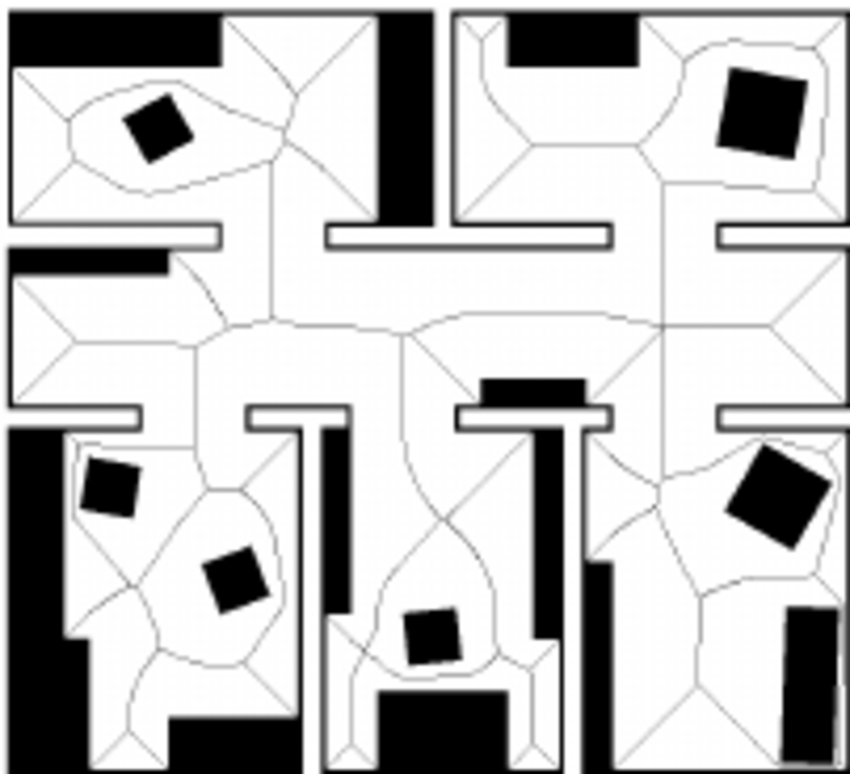
\includegraphics[width=0.5\textwidth]{./images/chapter3/gvd.png}
    \caption{GVD διδιάστατου χώρου}
    \label{fig:gdv_example}
\end{figure}

\section{Αλγόριθμος Brushfire}
\label{section:brushfire_theory}

Ο αλγόριθμος \emph{Brushfire} ή \emph{Wavefront} είναι μια μέθοδος υπολογισμού  αποστάσεων μεταξύ σημείων σε έναν διακριτοποιημένο χώρο σε μορφή γράφου, όπως ένα OGM. Ο αλγόριθμος εκκινεί από ένα σύνολο σημείων του χώρου και βρίσκει τα αμέσως γειτονικά τους σημεία επαναληπτικά. Έτσι υπολογίζει την κοντινότερη απόσταση κάθε σημείου του ελεύθερου χώρου από το αρχικό υποσύνολο σημείων κρατώντας το πλήθος των επαναλήψεων που χρειάστηκαν για να φτάσει εως εκεί. Στην παρούσα διπλωματική η διαδικασία αυτή χρησιμοποιείται σε διάφορες παραλλαγές, ενώ σημειώνεται ότι σε όλες τις περιπτώσεις έχει υλοποιηθεί σε γλώσσα C για την βελτίωση της ταχύτητας της διαδικασίας των υπολογισμών. 

Επιπλέον, ως γειτονικά σημεία κάθε σημείου του χώρου μπορούν να θεωρηθούν είτε μόνο τα τέσσερα σημεία (βόριο, νότιο, ανατολικό και δυτικό) που παρουσιάζονται στο \autoref{fig:brushfire_neighbors_matrix} με πράσινο χρώμα είτε και τα οκτώ σημεία που βρίσκονται γύρω του. Στην μελέτη αυτή χρησιμοποιήθηκαν και τα 8 σημεία ως γείτονες σε όλες τις περιπτώσεις, καθώς έτσι προσεγγίζεται η πραγματική απόσταση μεταξύ σημείων με μεγαλύτερη ακρίβεια.

\begin{figure}[!htb]
    \centering
    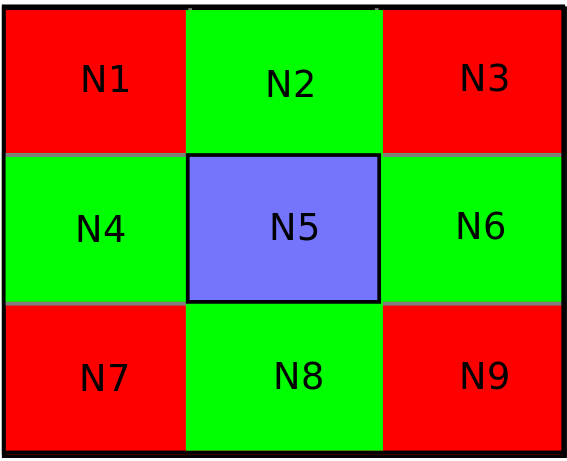
\includegraphics[width=0.3\textwidth]{./images/chapter3/neighbors2.png}
    \caption{Πίνακας γειτόνων σημείων}
    Πηγή: \href{http://roboscience.org/book/html/Planning/Brushfire.html}{http://roboscience.org/book/html/Planning/Brushfire.html}
    \label{fig:brushfire_neighbors_matrix}
\end{figure}

\section{Αλγόριθμός Dijkstra}
\label{section:dijkstra}


Ο αλγόριθμος \emph{Dijkstra} \cite{Dijkstra1959} είναι ένας αλγόριθμος εύρεσης του ελάχιστου μονοπατιού μεταξύ κόμβων ενός γράφου. Δέχεται ως είσοδο έναν γράφο, τον κόμβο αφετηρία και τον κόμβο στόχο και εκτελεί μια επαναληπτική διαδικασία εύρεσης της βέλτιστης διαδρομής από την αφετηρία μέχρι τον στόχο. Κριτήριο βελτιστοποίησης είναι η ελαχιστοποίηση του συνολικού κόστους του μονοπατιού, που αποτελείται από το άθροισμα των βαρών των ακμών της κάθε διαδρομής.

Ένας γράφος, για παράδειγμα, μπορεί να αναπαριστά διάφορες πόλεις μιας χώρας, οι ακμές του τους δρόμους που ενώνουν πόλεις μεταξύ τους και τα βάρη των ακμών τις αποστάσεις τους. Ο αλγόριθμος αυτός μπορεί να βρει την κοντινότερη διαδρομή από μια πόλη προς όλες τις υπόλοιπες.


Η πολυπλοκότητα του αλγορίθμου αυτόυ είναι $O$($|V|^2$), 
όπου $|V|$ είναι ο αριθμός των κόμβων.


\begin{algorithm}[!ht]
\caption{Dijkstra}
\label{alg:dijkstra}
\begin{algorithmic}[1]
    \Function{dijkstra}{Graph, source}
        \For{each vertex $v$ in $Graph$}
            \State $dist[v] = infinity$
            \State $previous[v] = undefined$
        \EndFor
        \State $dist[source] = 0$
        \State $Q = the\ set\ of\ all\ nodes\ in\ Graph$
        \While{$Q$ is not empty}
            \State $u = node\ in\ Q\ with\ smallest\ dist[]$
            \State $remove\ u\ from\ Q$
            \For{each neighbor $v$ of $u$}
                \State $alt = dist[u] + dist\_between(u,v)$
                \If{$alt < dist[v]$}
                    \State $dist[v] = alt$
                    \State $previous[v] = u$
                \EndIf
            \EndFor
        \EndWhile
        \State \Return $previous[]$
\end{algorithmic}
\end{algorithm}

\section{Αλγόριθμός Hill Climbing}
\label{section:hill_climbing}

O αλγόριθμος \emph{ανάβασης πλαγιάς} (Hill Climbing - HC)\footnote{\href{https://en.wikipedia.org/wiki/Hill_climbing}{https://en.wikipedia.org/wiki/Hill\_climbing}} είναι μια τεχνική βελτιστοποίησης που ανήκει στην κατηγορία της τοπικής αναζήτησης της αριθμητικής ανάλυσης. Είναι ένας επαναληπτικός αλγόριθμος που ξεκινάει με μία αυθαίρετη λύση στο πρόβλημα που μελετάται και προσπαθεί να βρει συνεχώς μια καλύτερη αλλάζοντας στοιχειωδώς την λύση. Εαν κάποια αλλαγή οδηγεί σε καλύτερο αποτέλεσμα, τότε η λύση αυτή κρατείται ως η τρέχουσα βέλτιστη και η διαδικασία συνεχίζεται με μια επόμενη αλλαγή. Η διαδικασία τερματίζεται όταν σταματήσει να υπάρχει κάποια αλλαγή που να βελτιώνει την τρέχουσα λύση. 

Ο αλγόριθμος αυτός βρίσκει την καλύτερη δυνατή λύση του προβλήματος μέσα σε μια τοπική περιοχή, που εξαρτάται αποκλειστικά από την αρχική αυθαίρετη λύση. Αυτό σημαίνει ότι ο αλγόριθμος μπορεί να εγκλωβιστεί σε τοπικά μέγιστα, δίχως να μπορεί να προσεγγίσει τα ολικά μέγιστα. Ωστόσο, το γεγονός ότι είναι πολύ απλός και γρήγορος στην υλοποίηση του τον καθιστούν χρήσιμο σε προβλήματα που ο χρόνος υπολογισμού είναι σημαντικός ή σε προβλήματα που η ολική λύση δεν απέχει σημαντικά από τις τοπικές.

Ταυτόχρονα, έχουν δημιουργηθεί διάφορες παραλλαγές του, με στόχο την αποφυγή του σημαντικού αυτού μειονεκτήματος που έχει. Δύο τέτοιες παραλλαγές χρησιμοποιήθηκαν σε αυτή την διπλωματική εργασία. Στην πρώτη παραλλαγή χρησιμοποιούνται επανεκκινήσεις της διαδικασίας όταν αυτή κολλάει σε τοπικά μέγιστα (Random Restart Hill Climbing - RRHC)\footnote{\href{https://en.wikipedia.org/wiki/Hill_climbing#Variants}{https://en.wikipedia.org/wiki/Hill\_climbing#Variants}}. Πιο αναλυτικά, εκτελείται ο απλός αλγόριθμος hill climbing μέχρι να φτάσει σε ένα τοπικό μέγιστο, όπου και η λύση αυτή κρατείται. Στη συνέχεια, εκτελείται ξανά ο hill climbing με διαφορετική αρχική λύση. Έτσι, εαν το νέο τοπικό μέγιστο αποτελεί βελτίωση του προηγούμενου, το αντικαθιστά. Η διαδικασία αυτή επαναλαμβάνεται για έναν συγκεκριμένο αριθμό επαναλήψεων που έχουν ορισθεί στην αρχή της διαδικασίας. Η δεύτερη παραλλαγή χρησιμοποιεί μια στοχαστική πιθανότητα για να αποδέχεται και αλλαγές που δεν βελτιώνουν την τρέχουσα λύση. Αυτή δίνει την δυνατότητα αποφυγής ορισμένων τοπικών ακρότατων, καθώς η λύση δεν περιορίζεται σε μια μικρή περιοχή τιμών. Μάλιστα, η πιθανότητα αυτή συνήθως με το πέρασμα των επαναλήψεων τείνει να μεταβάλλεται με τρόπο τέτοιο, ώστε ο αλγόριθμος να δέχεται όλο και περισσότερες αλλαγές που βελτιώνουν αυστηρά την λύση, προσεγγίζοντας σε άπειρο χρόνο την αρχική εκδοχή του hill climbing.


% \section{Support Vector Machines}
\label{section:svm}

Στον κλάδο της μηχανικής μάθησης υπάρχουν πολλοί διαφορετικοί αλγόριθμοι δημιουργίας μοντέλων πρόβλεψης. Μια κατηγορία τέτοιων μοντέλων είναι τα SVM, τα οποία χρησιμοποιούνται στην επιβλεπόμενη μάθηση και περιέχουν αλγορίθμους ανάλυσης των δεδομένων που αφορούν προβλήματα ταξινόμησης και παλινδρόμησης. Το σύνολο δεδομένων αποτελείται από δείγματα που περιέχουν τιμές από ορισμένες μεταβλητές, τα χαρακτηριστικά τους, και μια κλάση στόχο, στην οποία αντιστοιχεί το κάθε δείγμα. Συνήθως χρησιμοποιούνται σε δυαδικά προβλήματα ταξινόμησης, όπου η κλάση στόχος παίρνει τις τιμές ΝΑΙ και ΟΧΙ ή 1 και 0. Στόχος των μοντέλων αυτών είναι να προβλέψουν την κλάση ενός νέου άγνωστου δείγματος, χρησιμοποιώντας μόνο τις τιμές από τα χαρακτηριστικά του. Ένα τέτοιο παράδειγμα παρουσιάζεται στο \ref{fig:svm_example}, όπου και τα διάφορα δείγματα περιέχουν δύο χαρακτηριστικά και διαχωρίζονται από το μοντέλο με την πράσινη ευθεία - όριο σε δύο χώρους, ανάλογα με την κλάση τους. Οι δύο κλάσεις για οπτικούς λόγους εμφανίζονται με διαφορετικό χρώμα σε κάθε δείγμα.

Τα μοντέλα SVM προσπαθούν να συσχετίσουν τις τιμές των δειγμάτων με τις κλάσεις τους, αναλύωντας τον χώρο τιμών των διάφορων μεταβλητών. Συμπεριφέρονται στα δεδομένα σαν σημεία στον Ν-διάστατο χώρο και προσπαθούν να διαχωρίσουν τον χώρο αυτό σε δύο χώρους, έναν για κάθε κλάση, βρίσκοντας το βέλτιστο υπερεπίπεδο διαχωρισμού. Έτσι, κάθε νέο δείγμα που εμφανίζεται, εισέρχεται στον χώρο αυτό και το μοντέλο ελέγχει σε ποιον από τους δύο χώρους ανήκει, στον οποίο και ταξινομείται.


\begin{figure}
    \centering
    \includegraphics[width=0.5\textwidth]{./images/chapter3/svm_example.png}
    \caption{Διαχωρισμός χώρου με μοντέλο SVM}
    Πηγή: \href{https://eight2late.wordpress.com/2017/02/07/a-gentle-introduction-to-support-vector-machines-using-r/}{https://eight2late.wordpress.com/2017/02/07/a-gentle-introduction-to-support-vector-machines-using-r/}
    \label{fig:svm_example}
\end{figure}

Ο διαχωρισμός του Ν-διάστατου χώρου γίνεται γραμμικά, ωστόσο υπάρχουν μέθοδοι προσέγγισης και μη γραμμικών προβλημάτων με SVM μοντέλα χρησιμοποιώντας τους λεγόμενους πυρήνες. Οι πυρήνες αυτοί μετασχηματίζουν τα δεδομένα με τέτοιον τρόπο, ώστε το μετασχηματισμένο σύνολο τιμών να είναι γραμμικώς διαχωρίσιμο.

Στην παρούσα διπλωματική εργασία γίνεται χρήση ενός γραμμικού SVM μοντέλου για την ταξινόμηση του κάθε χώρου σε δωμάτιο ή διάδρομο.

